\documentclass[a4paper]{article}
\usepackage[utf8]{inputenc}
\usepackage[spanish, es-tabla, es-noshorthands]{babel}
\usepackage[table,xcdraw]{xcolor}
\usepackage[a4paper, footnotesep = 1cm, width=20cm, top=2.5cm, height=25cm, textwidth=18cm, textheight=25cm]{geometry}
%\geometry{showframe}

\usepackage{tikz}
\usepackage{amsmath}
\usepackage{amsfonts}
\usepackage{amssymb}
\usepackage{float}
\usepackage{graphicx}
\usepackage{caption}
\usepackage{subcaption}
\usepackage{multicol}
\usepackage{multirow}
\setlength{\doublerulesep}{\arrayrulewidth}
\usepackage{booktabs}

\usepackage{hyperref}
\hypersetup{
    colorlinks=true,
    linkcolor=blue,
    filecolor=magenta,      
    urlcolor=blue,
    citecolor=blue,    
}

\newcommand{\quotes}[1]{``#1''}
\usepackage{array}
\newcolumntype{C}[1]{>{\centering\let\newline\\\arraybackslash\hspace{0pt}}m{#1}}
\usepackage[american]{circuitikz}
\usetikzlibrary{calc}
\usepackage{fancyhdr}
\usepackage{units} 
\usepackage{svg}

\graphicspath{{../Ejercicio-1/}{../Ejercicio-2/}{../Ejercicio-3/}{../Ejercicio-4/}{../Ejercicio-5/}}
%\svgpath{{../Ejercicio-1/}{../Ejercicio-2/}{../Ejercicio-3/}{../Ejercicio-4/}{../Ejercicio-5/}}

\pagestyle{fancy}
\fancyhf{}
\lhead{22.05 ASSD}
\rhead{Mechoulam, Lambertucci, Rodriguez, Londero}
\rfoot{Página \thepage}

\begin{document}

%%%%%%%%%%%%%%%%%%%%%%%%%
%		Caratula		%
%%%%%%%%%%%%%%%%%%%%%%%%%

%\begin{titlepage}
\newcommand{\HRule}{\rule{\linewidth}{0.5mm}}
\center
\mbox{\textsc{\LARGE \bfseries {Instituto Tecnológico de Buenos Aires}}}\\[1.5cm]
\textsc{\Large 22.99 Laboratorio de microprocesadores}\\[0.5cm]


\HRule \\[0.6cm]
{ \Huge \bfseries Trabajo práctico N$^{\circ}$N}\\[0.4cm] 
\HRule \\[1.5cm]


{\large

\emph{Grupo 3}\\
\vspace{3px}

\begin{tabular}{lr} 	
\textsc{Mechoulam}, Alan  &  58438\\
\textsc{Lambertucci}, Guido Enrique  & 58009 \\
\textsc{Rodriguez Turco}, Martín Sebastian  & 56629 \\
\textsc{Londero Bonaparte}, Tomás Guillermo  & 58150 \\
\end{tabular}

\vspace{20px}

\emph{Profesores}\\
Jacoby, Daniel Andres\\
Magliola, Nicolas\\
Ismirlian, Diego Matías\\

\vspace{3px}
%\textsc{} \\	

\vspace{100px}

\begin{tabular}{ll}

Presentado: & 18/08/20\\

\end{tabular}

}

\vfill

\end{titlepage}


%%%%%%%%%%%%%%%%%%%%%
%		Indice		%
%%%%%%%%%%%%%%%%%%%%%

\tableofcontents
\newpage

%%%%%%%%%%%%%%%%%%%%%
%		Informe		%
%%%%%%%%%%%%%%%%%%%%%

\section{Introducción}
	\label{intro}
	\subsection{Implementación por lógica discreta}
Para la lógica combinacional lo primero que se hizo fue escribir las posiciones de memoria en las que vivirá nuestro periférico en binario, teniendo en cuenta que la memoria es de 8KiB (8192 bytes) ocupará 0x2000 posiciones de memoria.
\begin{table}[H]
\centering
\begin{tabular}{cccc}
\hline
\textbf{Address} & \textbf{Dispositivo} & \textbf{Binario Comienzo} & \textbf{Binario Fin} \\ \hline
0x4000 & RAM & 010000000000 & 011000000000 \\ \hline
\end{tabular}
\caption{Parámetros de la memoria RAM.}
\end{table}
De aqui se arma la tabla de verdad de los últimos 3 bits mas significativos.
\begin{table}[H]
\centering
\begin{tabular}{cccc}
\hline
$\mathbf{a_{15}}$ & $\mathbf{a_{14}}$ & $\mathbf{a_{13}}$ & \textbf{CS} \\ \hline
0 & 0 & 0 & 0 \\
0 & 0 & 1 & 0 \\
0 & 1 & 0 & 1 \\
0 & 1 & 1 & 1 \\
1 & 0 & 0 & 0 \\
1 & 0 & 1 & 0 \\
1 & 1 & 0 & 0 \\
1 & 1 & 1 & 0	\\ \hline
\end{tabular}
\caption{Tabla de verdad.}
\label{tab:truetab}

\end{table}
De aquí se puede solucionar el mapa de karnaugh para la siguiente configuración:
\begin{figure}[H]
  \centering
  \includegraphics[width=0.5\textwidth,page = 1]{ImagenesEjercicio1/Circuits.pdf}
  \caption{Lógica Discreta.}
  \label{fig:circLog}
\end{figure}
\subsection{Implementación por lógica de baja complejidad}
Se utilizó el decodificador 74LS139, conectando a los pines $a_{15}$ y $a_{14}$ a las entradas B y A respectivamente, el CS será la salida $Y_1$ quedando de la siguiente manera
\begin{figure}[H]
  \centering
  \includegraphics[width=0.5\textwidth,page = 2]{ImagenesEjercicio1/Circuits.pdf}
  \caption{Lógica de baja complejidad.}
  \label{fig:circdec}
\end{figure}
\subsection{Implementación por medio de una PAL}
Se utilizó una PAL como decodificador de direcciones, como se observa en la Tabla (\ref{tab:truetab}) es posible detectar el perisferico viendo únicamente los bits $a_{15}$ y $a_{14}$ asi se llega a la siguiente ecuación:
\begin{align}
x_1 = a_{15} \ \ \  \  \  \  \  \  \  \ x_2=a_{14} \\
f1=CS \ \ \ f1= \bar{x_1} \  \&  \ x_2
\end{align}

\subsection{Análisis y construcción del diagrama de tiempos}
Se construyó para el microprocesador M68HC11 el diagrama de tiempos para un ciclo de lectura/escritura, usando como ejemplo la posición de memoria \$2345, la cual está dentro de la hipotética región del mapa de memoria donde se aloja la memoria para la cual se diseñó el decodificador anteriormente.

\begin{figure}[H]
  \centering
  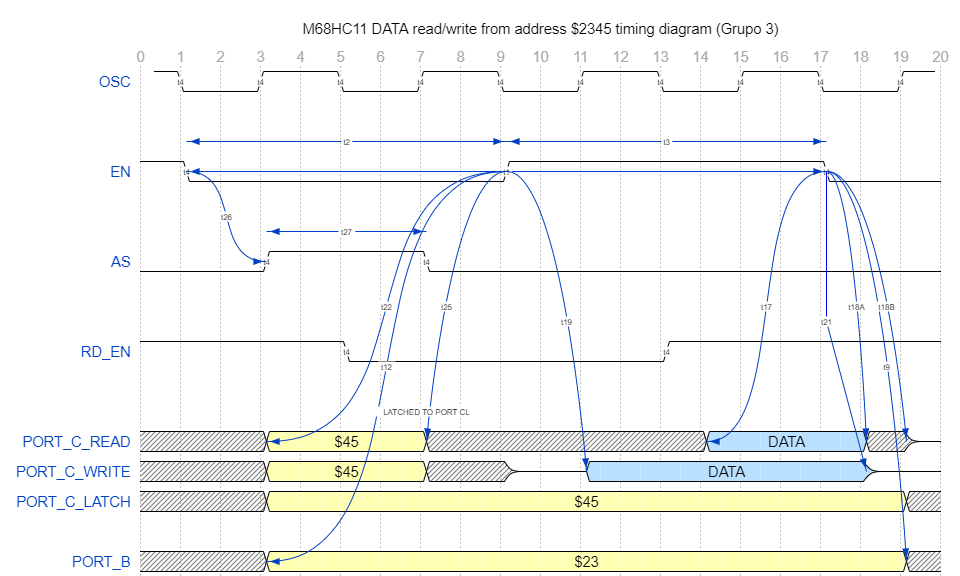
\includegraphics[width=\textwidth]{ImagenesEjercicio1/diagtiempos.png}
  \caption{Ciclo de lectura/escritura de \textit{DATA} en la dirección de memoria \textit{\$2345}}.
  \label{diagtiempos}
\end{figure}
 
Para el análisis de tiempos se tiene en cuenta una frecuencia característica de $2 \ MHz$. Dado esto, se obtiene un rise time de las señales de $t_4 = 20 \ ns$ y un periodo entre ciclos de lectura/escritura de $t_1 = 500 \ ns$, por lo que los tiempos en alto y bajo de la señal \textbf{E} de enable serán de $t_3 = 230 ns$ respectivamente. 

\subsubsection{Primera mitad del ciclo de escritura/lectura}

El comienzo del ciclo de lectura o escritura comienza con el flanco descendente de la señal de enable. Un tiempo $t_{26} = 53 \ ns$ después se activa la señal \textbf{AS} de address strobe, lo cual indica que se comienza a cargar el bus de address. Por un lado la parte baja y por otro la parte alta de la dirección de memoria en los puertos C y B del M68HC11 respectivamente. Esta señal se desactiva luego de un tiempo $t_{27} = 96 \ ns$ activando el latch que retendrá la parte baja de la dirección de memoria. De esta manera se logra multiplexar en el tiempo el bus de datos (puerto C) la parte baja del bus de address. Esto nos permite reutilizar los pines del puerto C para leer o escribir datos al igual que establecer la parte baja de la dirección del mapa de memoria.

El puerto C tiene la dirección de memoria por un tiempo válido de $t_{22} = 88 \ ns$ como mínimo y el puerto B por un tiempo de $t_{12} = 94 \ ns$ como mínimo, que corresponde con el flanco ascendente de la señal \textbf{E} de enable y marca la mitad del ciclo de lectura/escritura.

\subsubsection{Segunda mitad del ciclo de escritura/lectura} 
\textbf{Lectura:}
En el caso de la lectura, el tiempo de setup para que el periférico coloque el dato a su salida y lo mantenga estable antes del flanco descendente de la señal \textbf{E} de enable es de $t_{17} = 30 \ ns$ y debe ser mantenido estable por $t_{18A} = 10 \ ns$ pasado dicho flanco. Luego el puerto C pasa a modo de alta impedancia pasados $t_{18B} = 83 \ ns$ de dicho flanco.

\textbf{Escritura:}
Para el caso de la escritura, el puerto C tiene un delay máximo para contener el dato a escribir de $t_{19} = 128 \ ns$ y un tiempo de hold de $t_{21} = 33 \ ns$ como mínimo, por lo cual el tiempo de escritura deberá ser como máximo de $t_{3} + t_{21} - t_{19} = 143 \ ns$.

Finalmente, el address se mantendrá por un tiempo de $t_9$ tras el flanco descendente de la señal \textbf{E} de enable, por lo que el tiempo válido de lectura de la dirección de memoria en un ciclo de $t_1 = 500ns$ será de $t_1 - t_{26} + t_{9} = 480 \ ns$.

\section{Implementación}
	\subsection{Maquina de estados}
	\label{imp}
	\documentclass[a4paper]{article}
\usepackage[utf8]{inputenc}
\usepackage[spanish, es-tabla, es-noshorthands]{babel}
\usepackage[table,xcdraw]{xcolor}
\usepackage[a4paper, footnotesep = 1cm, width=20cm, top=2.5cm, height=25cm, textwidth=18cm, textheight=25cm]{geometry}
%\geometry{showframe}

\usepackage{tikz}
\usepackage{amsmath}
\usepackage{amsfonts}
\usepackage{amssymb}
\usepackage{float}
\usepackage{graphicx}
\usepackage{caption}
\usepackage{subcaption}
\usepackage{multicol}
\usepackage{multirow}
\setlength{\doublerulesep}{\arrayrulewidth}
\usepackage{booktabs}

\usepackage{hyperref}
\hypersetup{
    colorlinks=true,
    linkcolor=blue,
    filecolor=magenta,      
    urlcolor=blue,
    citecolor=blue,    
}

\newcommand{\quotes}[1]{``#1''}
\usepackage{array}
\newcolumntype{C}[1]{>{\centering\let\newline\\\arraybackslash\hspace{0pt}}m{#1}}
\usepackage[american]{circuitikz}
\usetikzlibrary{calc}
\usepackage{fancyhdr}
\usepackage{units} 
\usepackage{svg}

\graphicspath{{../Ejercicio-1/}{../Ejercicio-2/}{../Ejercicio-3/}{../Ejercicio-4/}{../Ejercicio-5/}}
%\svgpath{{../Ejercicio-1/}{../Ejercicio-2/}{../Ejercicio-3/}{../Ejercicio-4/}{../Ejercicio-5/}}

\pagestyle{fancy}
\fancyhf{}
\lhead{22.05 ASSD}
\rhead{Mechoulam, Lambertucci, Rodriguez, Londero}
\rfoot{Página \thepage}

\begin{document}
Para este ejercicio se implemento el decodificador de direcciones con un integrado 74LS138 y lógica combinacional.
Valiendonos de que dado a que únicamente se utilizaran estos 4 periféricos es posible asignar cantidades de memoria por demás a los periféricos.
quedando de la siguiente manera la tabla de direcciones.
\begin{table}[H]
\centering
\begin{tabular}{|c|c|c|c|}
\hline
Adress & Dispositivo & Binario Comienzo & Binario Fin \\ \hline
C000 & ROM16K & 1100000000000000 & 1111111111111111 \\ \hline
A800 & Entrada 8 Bits & 1010100000000000 & 1011111111111111 \\ \hline
A000 & Salida 8 Bits & 1010000000000000 & 1010011111111111 \\ \hline
2000 & RAM4K & 0010000000000000 & 0010111111111111 \\ \hline
\end{tabular}
\end{table}
Basta con conectar los siguientes bits con el decoder
\begin{align}
a_{14} \implies C\\
a_{15} \implies B\\
a_{11} \implies A
\end{align}
así también conectar las salidas $Y_0$ $Y_1$  con una compuerta or, al igual que las $Y_6$ $Y_7$ con otra.
quedando definidos los chip select de la siguiente manera.

\begin{figure}[H]
  \centering
  \includegraphics[width=.6\textwidth, page = 1]{ImagenesEjercicio2/Circuits.pdf}
  \caption{Diagrama en bloques}.
  \label{fig:fotofea}
\end{figure}

\end{document}
	
	\subsection{Capas e interfaces}
	\label{drivers}
	\documentclass[a4paper]{article}
\usepackage[utf8]{inputenc}
\usepackage[spanish, es-tabla, es-noshorthands]{babel}
\usepackage[table,xcdraw]{xcolor}
\usepackage[a4paper, footnotesep = 1cm, width=20cm, top=2.5cm, height=25cm, textwidth=18cm, textheight=25cm]{geometry}
%\geometry{showframe}

\usepackage{tikz}
\usepackage{amsmath}
\usepackage{amsfonts}
\usepackage{amssymb}
\usepackage{float}
\usepackage{graphicx}
\usepackage{caption}
\usepackage{subcaption}
\usepackage{multicol}
\usepackage{multirow}
\setlength{\doublerulesep}{\arrayrulewidth}
\usepackage{booktabs}

\usepackage{hyperref}
\hypersetup{
    colorlinks=true,
    linkcolor=blue,
    filecolor=magenta,      
    urlcolor=blue,
    citecolor=blue,    
}

\newcommand{\quotes}[1]{``#1''}
\usepackage{array}
\newcolumntype{C}[1]{>{\centering\let\newline\\\arraybackslash\hspace{0pt}}m{#1}}
\usepackage[american]{circuitikz}
\usetikzlibrary{calc}
\usepackage{fancyhdr}
\usepackage{units} 
\usepackage{svg}

\graphicspath{{../Ejercicio-1/}{../Ejercicio-2/}{../Ejercicio-3/}{../Ejercicio-4/}{../Ejercicio-5/}}
%\svgpath{{../Ejercicio-1/}{../Ejercicio-2/}{../Ejercicio-3/}{../Ejercicio-4/}{../Ejercicio-5/}}

\pagestyle{fancy}
\fancyhf{}
\lhead{22.05 ASSD}
\rhead{Mechoulam, Lambertucci, Rodriguez, Londero}
\rfoot{Página \thepage}

\begin{document}

\subsection{Introducción}

\end{document}

%\section{Ejercicio 4}
%	\label{Ejercicio-4}
%	\begin{center}
\textcolor{black}{\huge{\textbf{\underline{Manual de usuario}}}}
\end{center}

\begin{center}
\textbf{\LARGE{Inicio:}}
\end{center}

Al encender el dispositivo, se esperará que se ingrese un ID (8 dígitos), utilizando el encoder (rotandolo para seleccionar los números y con el botón del mismo validando el caracter) ó la tarjeta. En caso de que la ID introducida no sea correcta titilará el led \textcolor{red}{rojo} de la FRDM. Una vez ingresada la ID, titilará el led \textcolor{blue}{azul} y deberá ingresar el PIN (5 dígitos). Con el botón del \textbf{CANCEL} (SW2) se puede cancelar la introducción del PIN/ID, mientras que con el \textbf{BACK} (SW3) se vuelve al anterior.

Se cuenta con 3 intentos para ingresar dicho pin. En el caso de que el introducido no sea correcto titilará el led \textcolor{red}{rojo}. Luego de los 3 intentos fallidos, se bloqueará dicho ID, hasta que un \textbf{ADMIN} lo añada de vuelta.

En el caso de inactividad, es decir, que no se efectúe ninguna acción, se volverá al menú de inicio automáticamente, deslogueando al usuario, sin importar en que submenú se encuentre el usuario.

\begin{center}
\textbf{\LARGE{Access:}}
\end{center}

Una vez dentro es posible navegar a través de las distintas opciones mediante el uso del encoder. Las opciones disponibles son ``OPEN'', ``USERS'' y ``BRIGHT''. Open permite abrir la puerta durante 5 segundos. En este intervalo titilará el led \textcolor{green}{verde} y aparecerá un mensaje de ``OPEN DOOR'' en el display. Por otro lado, las otras dos opciones permiten configurar el sistema.

\begin{center}
\textbf{\LARGE{Menúes:}}
\end{center}

\textbf{\Large{Brightness:}}


Permite configurar el nivel de brillo del display, existiendo 3 distintos niveles.

\vspace*{0.5cm}

\textbf{\Large{Users:}}

En este puede configurarse 3 opciones distintas, de las cuales dos son exclusivas para administradores.

\vspace*{0.25cm}
\textbf{\large{Clave:}}
En este submenu, disponible para cualquier usuario, permite cambiar el PIN de seguridad del usuario. Este debe introducirse mediante el uso del encoder.

\vspace*{0.25cm}
\textbf{\large{Delete:}}
\textbf{SOLO PARA ADMINS.} Se muestran en pantalla los distintos ID's disponibles en la base de datos. Gire para cambiar de ID y presione para eliminar.

\vspace*{0.25cm}
\textbf{\large{Add:}}
\textbf{SOLO PARA ADMINS.} En este submenu permite agregar usuarios nuevos a la base de datos, usando tanto el encoder como la tarjeta para agregar el ID pero solo el primero para agregar el PIN.

\begin{center}
\textbf{\LARGE{Consideraciones:}}
\end{center}

El sistema se alimenta con $3.3 \ V$.

%\section{Ejercicio 5}
%	\label{Ejercicio-5}
%	Se quiere construir el diagrama de tiempos del MC68HC11 para el programa de la Tabla (\ref{prog}).

\begin{table}[H]
\centering
\begin{tabular}{|cccc|}
\hline
 & org & $\$C000$ &  \\
 & ldaa &  & $\#\$A5$ \\
L1 & staa &  & $\$4000$ \\
 & jmp &  & L1 \\
 \hline
\end{tabular}
\caption{Programa a implementar.}
\label{prog}
\end{table}

Para esto, se construye la Tabla (\ref{prog1}) donde se descompone a cada instrucción en los ciclos que la componen.

\begin{table}[H]
\centering
\begin{tabular}{|cccc|}
\hline
Instruction & Cycle & Address & Data \\
LDAA & $1$ & $\$C000$ & $\$86$ \\
$$ & $2$ & $\$C001$ & $\$A5$ \\
STAA & $3$ & $\$C002$ & $\$B7$ \\
$$ & $4$ & $\$C003$ & $\$40$ \\
$$ & $5$ & $\$C004$ & $\$00$ \\
$$ & $6$ & $\$4000$ & $\$A5$ \\
JMP & $7$ & $\$C005$ & $\$7E$ \\
$$ & $8$ & $\$C006$ & $\$C0$ \\
$$ & $9$ & $\$C007$ & $\$02$ \\
\hline
\end{tabular}
\caption{Descomposición en ciclos del programa a implementar.}
\label{prog1}
\end{table}

Finalmente, se construye el diagrama de tiempos teniendo en cuenta el modo extendido del MC68HC11 en el cual el bus de address está compuesto por el puerto C para los ocho bits menos significativos y el puerto B para los ocho bits más significativos. A su vez, el puerto C está multiplexado de manera tal que funcione como bus de datos en el semiciclo bajo de la señal de enable. 

\begin{figure}[H]
  \centering
  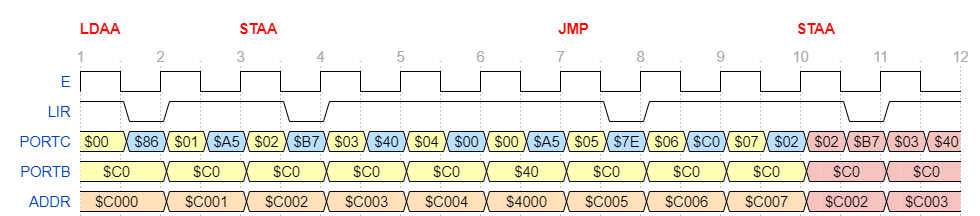
\includegraphics[width=\textwidth]{ImagenesEjercicio5/diagtiempos_5.png}
  \caption{Diagrama de tiempos del programa de la Tabla \ref{prog}.}
  \label{diagtiempos_5}
\end{figure}

La señal de ADDR indica el valor del bus de address visto como la concatenación del puerto C latcheado y el puerto B. La señal de LIR es una señal activa baja de ayuda al momento de debuggear y marca el primer semiciclo negativo de cada ciclo de cada nueva instrucción. Esto es útil debido a que, como se puede ver en la Figura (\ref{diagtiempos_5}), la señal LIR tendrá un valor bajo cuando el puerto C retiene el OPCODE, el cual identifica qué instrucción ejecutará el M68HC11.


\begin{center}
\textcolor{red}{\LARGE{Se debe agregar un pin de testeo (TP) que se encienda mientras se ejecutan las interrupciones, a fin de medir el tiempo que se emplea en la ISR y cuánto representa porcentualmente.}}
\end{center}


\end{document}